The TJ-Monopix1 is one of the chips fabricated by ToweJazz with 180 CMOS imaging process. From the middle of 2013 a dedicated collaboration, RD 53 ('Development of pixel readout integrated circuits for extreme rate and radiation'), has been estabilished with the specific goal to find a sensor suitable as vertex detector for future upgrade of CMS and ATLAS experiments. Among the main objects of study of the collaboration there are both hybrid pixels and monolitic options as CMOS MAPS: fig \ref{fig:TJ180nm} shows the intermediate MAPS-prototypes made by TowerJazz.\\
\begin{figure}[h!]
    \centering
    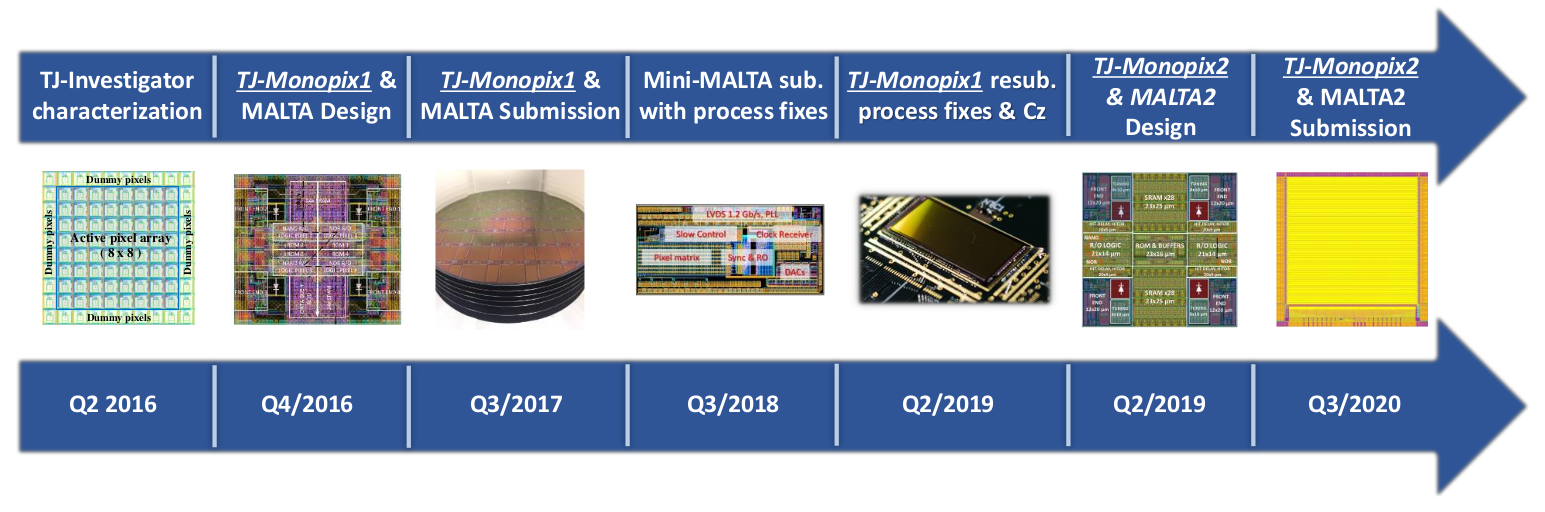
\includegraphics[width=.95\linewidth]{figures/Monopix1/TJ180nm.png}
    \caption{Timeline in TowerJazz productions.  In addition to Monopix serie also the small electrode demonstrator TJ-Malta and mini-Malta have been produced and tested\cite{MALTA}. The Malta prototypes differ from TJ-Monopix in the readout: while Monopix implements a column-drain R/O, an asynchronous R/O without any distribution of BCID has been used by TJ-Malta in order to reduce power consumption.}
    \label{fig:TJ180nm}
\end{figure} 
Besides the TowerJazz series, also LFoundry fabricated other similar sensors with 150 CMOSS technology~\cite{LF-Monopix}\cite{LF-TJ-Monopix}: LF-Monopix.\\
The main difference between the LFoundry and TowerJazz's products, summerized in \ref{tab:LF-TJ-Monopix}, is the sensor structure rather than the read out architecture, based on a column drain R/O with ToT capability (LF-Monopix has 8 bits dedicated and TJ-Monopix 6 bits). Concerning the sensor, LFoundry pixels are bigger and have a large-fill factor, while TJ-Monopix ones have a small fill-factor electrode.

The performances of both the detectors have been tested before and after irradiation ($\sim 10^{10} n_{eq}/cm^{2}$) and the result is, as expected since LF-Monopix is a large fill factor electrode (capitolo \ref{chap:}), that LF-Monopix is more radiation hard than TJ-Monopix whereas the main degradation of efficiency in TJ-Monopix chips is due to the low electic field in the pixel corner. On the other hand one more accidental consequence of the large fill factor size in LF-Monopix (the deep p-well covers $\sim$ 55 $\%$ of the pixel area) is a significant cross-talk problem.
\begin{table}
    \begin{center}
    \begin{tabular}{|c | c |c |}
    \hline
    & LF-Monopix1 & TJ-Monopix1\\
    \hline
    \hline
    Bulk & p-type substrate & p-epi. on a low $\rho$ substrate \\
    Resistivity & $maggiore$ 2k$\Omega$cm & maggiore 1k$\Omega$cm\\
    Pixel size & 50 x 250 $\mu m^2$ & 26x40 $\mu m^2$ \\
    Depth & 100-750 $\mu$m & 25 $\mu$m \\
    Capacity & $\sim$ 400 fF & $\sim$ 3 fF\\
    Preamplifier & CSA & Voltage \\
    Threshold trimming & on pixel (4-bit DAC) & global threshold\\
    Readout mode & Fast column drain & Fast column drain\\
    Consumption & $\sim$ 300 mW/$cm^2$& $\sim$ 120 mW/$cm^2$ \\
    Threshold & 1500 $e^-$ & $\sim$ 270 $e^-$ \\
    ENC & 100 $e^-$ & $\sim$ 30 $e^-$\\
    \hline
    \end{tabular}
    \caption{Main characteristics of TJ-Monopix and LF-Monopix \cite{LF-TJ-Monopix}}
    \label{tab:LF-TJ-Monopix}
    \end{center}
 \end{table}

\section{The sensor}
    TJ-Monopix1 adopts the modification described in \ref{chap:a_modified_sensor} that allows to achieve a planar depletion region near the electrode applying a relatively small reverse bias voltage: a low dose n implant is build on a high resistivity ($\geq $ 1 k$\Omega$ cm), p-type epitaxial layer.\\
    This modification improves the efficiency of the detector, especially after irradiation\cite{}; however a Technology Computer Aided Design (TCAD) simulation has shown that a nonuniform electric field is still produced in the lateral regions after the modification; since the transversal component of the electric field drops at the pixel corner (this point in figure \ref{fig:Monopix1_section_scheme} is indicated by a star) the efficiency at the side is reduced. \\
    On a sample of chip, the one I've tested in Pisa belongs to these, a second optimization have been made to enhance the lateral component of electric field and improve the efficiency and velocity in charge collection near the corners of the sensor: a portion of low dose implant has been removed, creating a step discontinuity in the pixel corner. 
    A side-effect is the weaker separation between the deep p-well and the p-substrate, that cannot be biased separately anymore to prevent the punchthrough. 
        \begin{figure}[h!]
        \centering
        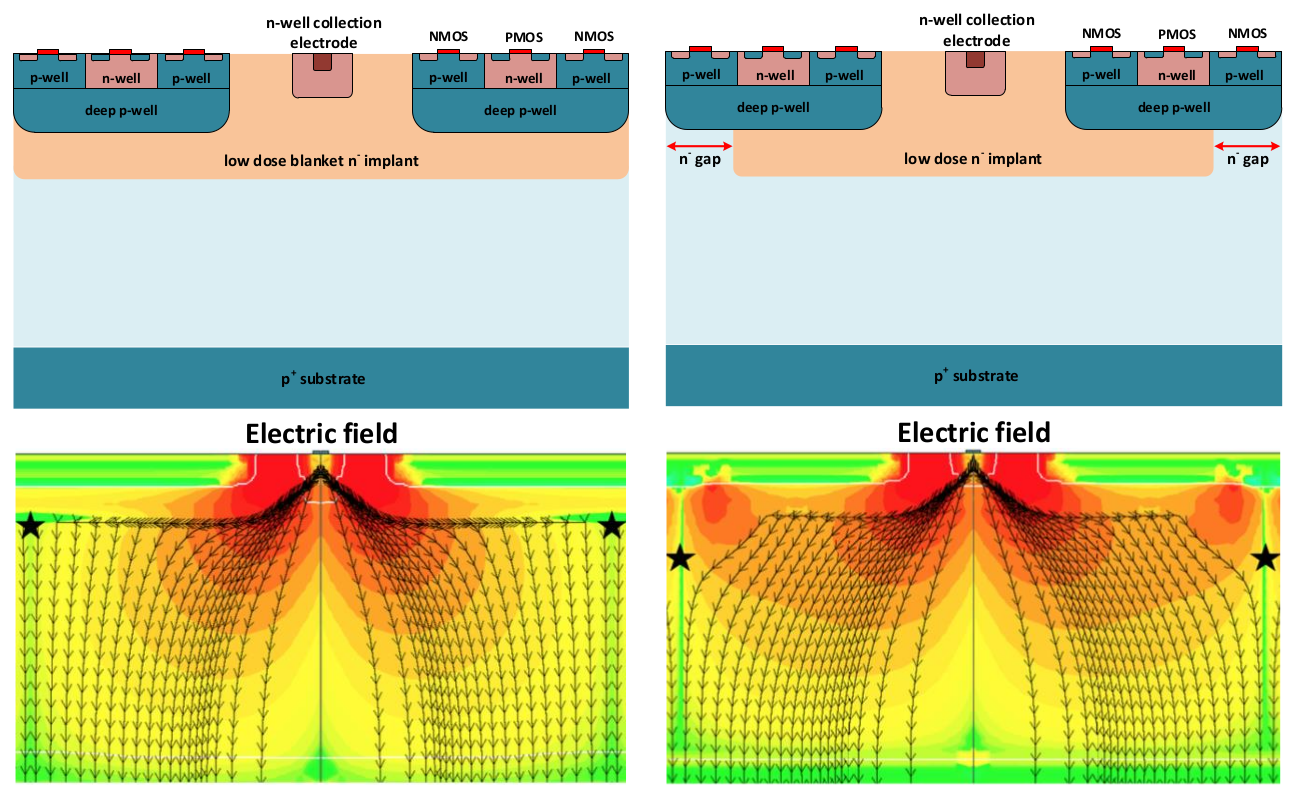
\includegraphics[width=.9\linewidth]{figures/Monopix1/Monopix1_section_scheme.png}
        \caption{(a) The cross-section of a monolithic pixel in the TJ-Monopix 180 nm with modified process; additionally in (b) a gap in the low dose implant is created to improve the collection of charge due to a bigger lateral component of the electric field}
        \label{fig:Monopix1_section_scheme}
    \end{figure}
    \begin{table}
        \begin{center}
        \begin{tabular}{| c |c |}
        \hline
        Parameter & Value\\
        \hline
        \hline
        Matrix size & \\
        Pixel size & 26x40 $\mu m^2$\\
        Depth & 25 $\mu$m \\
        BCID & 40 MHz \\
        ToT-bit & 6 \\
        Power consumption & $\sim$ 120 mW/$cm^2$\\
        \hline
        \end{tabular}
        \caption{}
        \label{tab:LF-TJ-Monopix}
        \end{center}
    \end{table}
    Moreover, to investigate the charge collection properties, as the threshold, the noise and the efficiency, pixels within the matrix feature a difference in the doping structure of the deep p-well: rows from 0 to 111 are fully covered by deep p-well (FDPW) under p-well near the sensor, while rows from 112 till the last 223 have a portion of deep p-well removed (RDPW). \\
    The removing enhance the lateral electric field component then resulting in a higher efficiency, as we'll see later.\\

\section{FE flavors}
    TJ-Monopix1 has been implemented in four different flavors, each one corresponding to a different sector on the matrix (fig. \ref{fig:Monopix1_flavors}) and thus having a separate readout and data trasmission, in order to explore different variations of the FE. The four flavors mainly differ in the reset input circuit.
    \begin{figure}[h!]
        \centering
        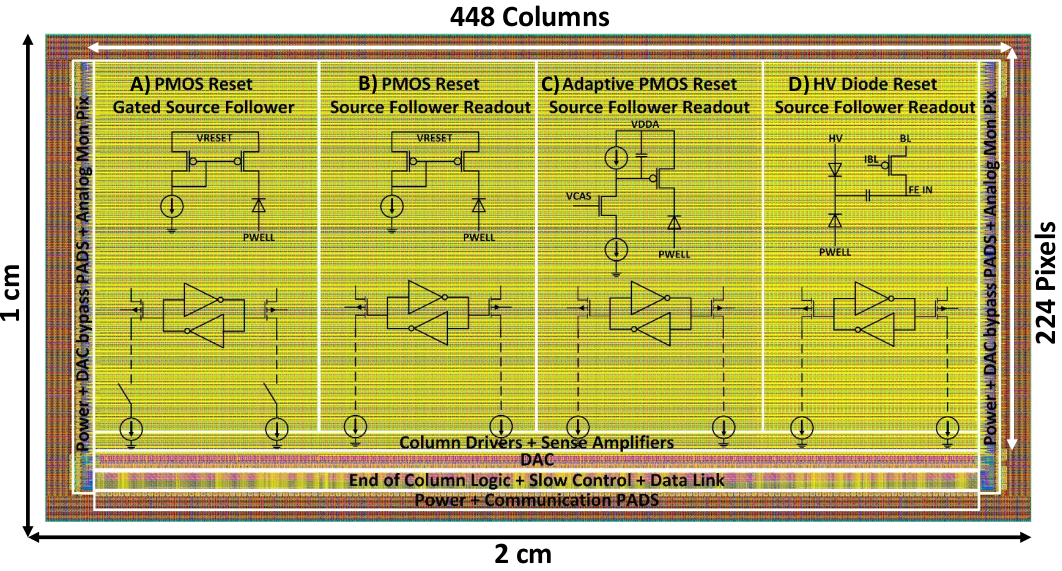
\includegraphics[width=.5\linewidth]{figures/Monopix1/Monopix1_flavors.png}
        \caption{}
        \label{fig:Monopix1_flavors}
    \end{figure}
    R resistenza di reset deve essere abbastanza grande in modo da far si che il ritorno allo zero è abbastanza lento (non devi "interferire" con la tot slope e non devi più corto del tempo del preamplificatore, sennò hai perdita di segnale).\\
    Baseline reset: all'input solitamente hai un PMOSS o un diodo;  

    The FE circuit \ref{fig:Monopix1_FE_circuit} is ALPIDE-like, so it is similar to the one described in \ref{chap:}; a quanto già detto voglio però aggiungere due parole: come viene implementato il mascheramento dei pixels e il reset.\\ 
    Prevedere un modo di mascherare gli screaming pixel, tipicamente pixels con manufacturing defects, è fondamentale per poter ridurre il rate molto alto di dati e non saturare la banda. 
    \begin{figure}[h!]
        \centering
        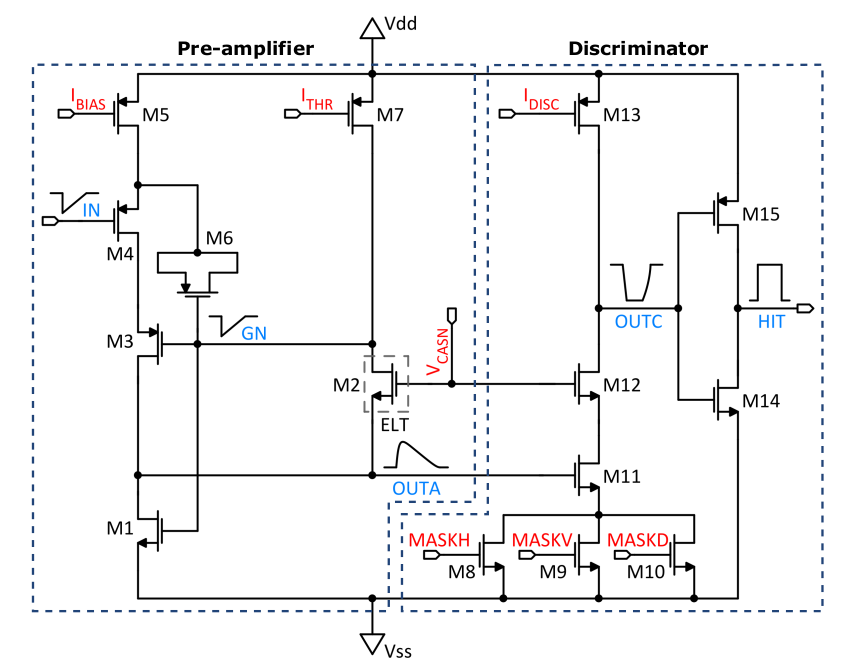
\includegraphics[width=.6\linewidth]{figures/Monopix1/Monopix1_FE_circuit.png}
        \caption{}
        \label{fig:Monopix1_FE_circuit}
    \end{figure}

    In the circuit in fig. \ref{fig:Monopix1_FE_circuit} transistors M8, M9 and M10 implement are used to disable pixels-readout, where MASKH, MASKV and MASKD represent respectivelly the vertical, orizontal and diagonal coordinates of the pixel that one want to mask. \\ 
    If all three transistors-signals are low, the discriminator is disabled and the pixel is masked. The masking is implemented in this way (with three cordinates instead of one) in order to avoid masking too many ghost pixels (fig. \ref{fig:masking_scheme}).
    \begin{figure}[h!]
        \centering
        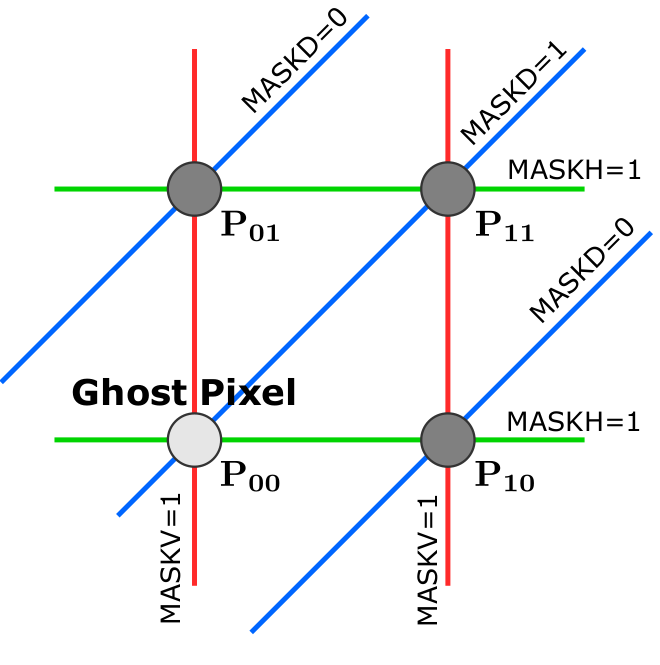
\includegraphics[width=.3\linewidth]{figures/Monopix1/masking_scheme.png}
        \caption{}
        \label{fig:masking_scheme}
    \end{figure}
    Un modo standard che si usa di solito è allocare un registro su ogni pixel periphery: il vantaggio di questo modo è che si può disabilitare ogni pixel individually. Questo metodo pur essendo più comodo richieda less amount of area ha però come drawback che il registro può essere soggetto a SEU \footnote{SEU = Single Event Upset, in sostanza è quando un bit ti cambia valore (da 0 a 1 o viceversa) perché una particella deposita carica nell'elettronica che fa da memoria (registro/RAM/...). Questo tipo di elettronica ha bisogno di un sacco di carica prima che il bit si "flippi" (cambi valore), infatti tipicamente per avere un SEU non basta una MIP che attraversa esattemente quel pezzo di chip in cui è implementata la memoria, ma un adrone che faccia interazione nucleare producendo più carica di quanto farebbe una MIP.} problema non trascurabile in acceleratori come HL-LHC adronici\\
    The implemented approch of masking in Monopix-1 funziona però solo se il numero di pixel da mascherare non è troppo alto dato che il numero di pixel unintentionally masked ("ghost pixels") increase with the number of pixels masked. \\
    Nel caso in cui solo due cordinate vengono utilizzate il numero di pixel unintentionally masked scales with $N^2$, where N is the number of the intentionally masked; if instead three coordinates are given the ghost pixels are $N^\alpha$ where $\alpha \min$2.\\

    \subsection{FE parameters}
    Descrivo un po' le misure fatte sul fe e sul significato dei vari parametri.\\
    \begin{table}
        \begin{center}
        \begin{tabular}{|c | c |}
        \hline
        Parameter & Meaning\\
        \hline
        \hline
        IBIAS\\
        IDB\\
        ITHR \\
        VCASN\\
        VREF\\
        IREF\\
        \hline
        \end{tabular}
        \caption{}
        \label{tab:FE-parameters}
        \end{center}
     \end{table}
    
\section{Readout logic}
    TJ-Monopix1 has a triggerless and fast R/O with ToT capability based on a column-drain architecture.      
    On the pixel are located two Random Access Memory (RAM) cells to store the 6-bit LE and 6-bit TE of the pulse and a Read-Only Memory (ROM) containing the 9-bit pixel address: excluded these memories, TJ-Monopix1 hasn't any other buffer.
    After being read, the data packet is sent to the EoC periphery of the chip, where a serializer transfer off-chip to an FPGA (\ref{fig.}). A FIFO is used to temporarily stored the data, which is after transmit to a computer through an ethernet cable.  
    \begin{figure}
        \begin{subfigure}{.5\textwidth}
        \centering
        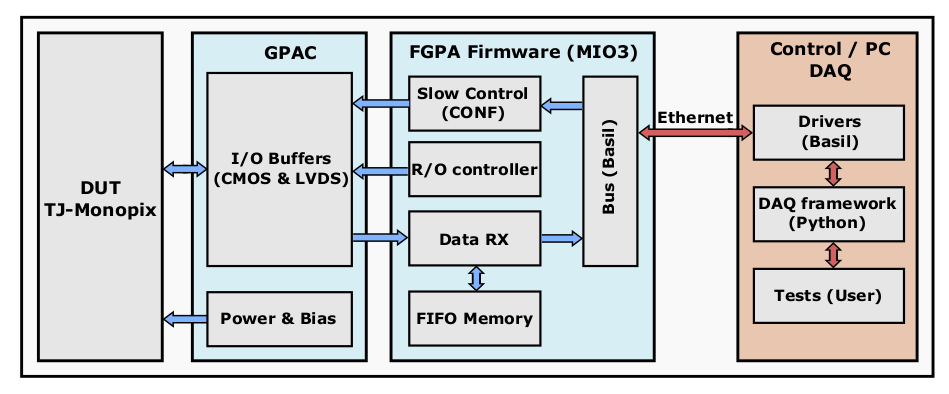
\includegraphics[width=.98\linewidth]{figures/Monopix1/schematic_boards.png}
        \end{subfigure}%
        \begin{subfigure}{.5\textwidth}
        \centering
        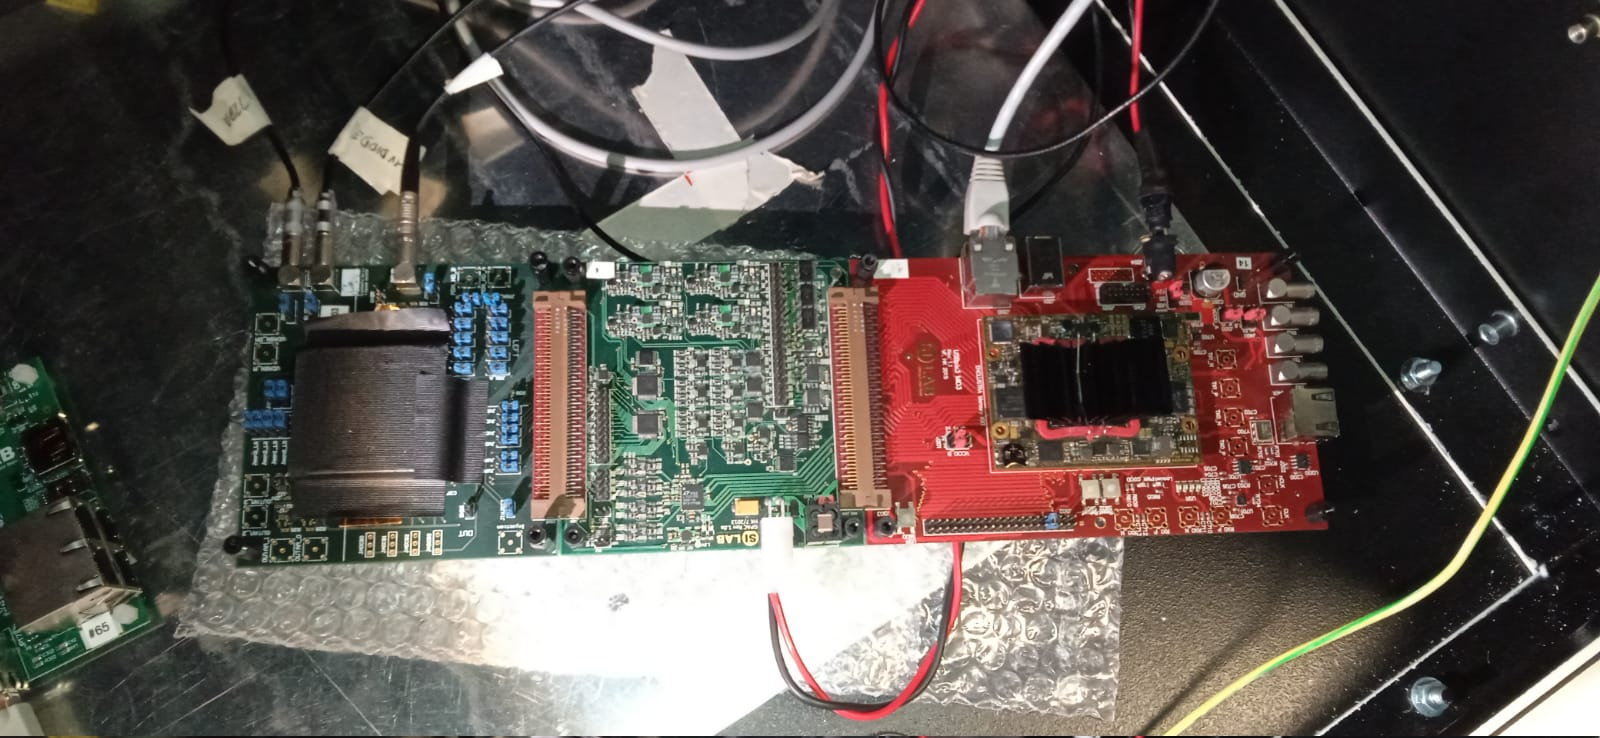
\includegraphics[width=.98\linewidth]{figures/Monopix1/monopix1_front.jpeg}
        \end{subfigure}
        \caption{(a) (b) From the left to the right: TJ-Monopix1, a breakout board used to make the reboot of data and the FPGA. \red{Dove sono state sviluppate BB e FPGA? Bonn?}}
        \label{fig:}
     \end{figure} 
  

    The access to the pixels' memory and the transmission of the data off-pixel is based on a Finite State Machine (FSM) composed by four state: no-operation (NOP), freeze (FRZ), read (RD) and data transfer (DTA). The readout sequence starts with the TE of a pulse: the pixel immediately tries to grab the column-bus turning up a hit flag signal called \textit{token}.   
    The token is used to control the priority chain and propagates across the column indicating the pixel that must be read. To start the readout and avoid that the arrival of new hits disrupt the priority logic, a \textit{freeze} signal is activated, and then a \textit{read} signal controls the readout and the access to memory.
    During the freeze, the token state of all pixels on the matrix remains settled: this does not forbid new hits from being recorded, but forbid pixels hit from turning on the token until the freeze is ended. 
    \red{The freeze is () fino a che il tokne non ha percorso tutta la priority chain and has reached the EoC, and only after that point is lowered. Until the freeze is applied . Supponiamo quindi che mentre la matrice sia freezata arrivino nuove hit. Quando il freeze si abbassa il token di queste hit si alza e il sistema di controllo si prepara a rialzaer il freeze; le hit che arrivano tra quando si è alzato il primo token e quando viene rialzato il freeze vengono lette. NON SO ANCORA COME SCRIVERLO BENE. È difficile da dire anche in italiano}
    Since the start of the token is used to assign a timestamp to the hit, the token time has a direct impact on the time assignation of the hit and therefore on the time resolution measurement. All the hits     
    
    \begin{figure}[h!]
        \centering
        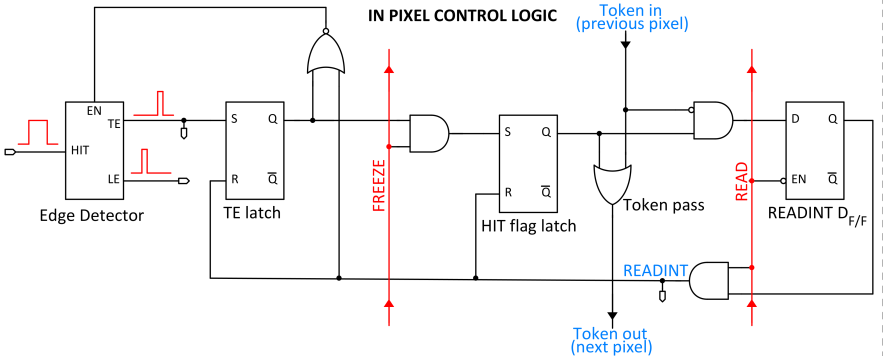
\includegraphics[width=.7\linewidth]{figures/Monopix1/Monopix1_readout_schematics.png}
        \caption{}
        \label{fig:Monopix1_readout_schematics}
    \end{figure}
    The data packet, that is long () bits, represents and contains all are information about the hit: the coordinates within the matrix and the ToT. Remembering that for each flavor there are 112 columns and 224 rows, and since the data bus are shared between double columns, to represent the data bus column () bits are needed, while the rows need () bits. 
    A 40 MHz BCID is distributed across the matrix with a simulated timing dispersion along a column of 0.1-0.2 ns. 


    \subsection{Dead time measurement}
        The RAM on pixel can store only one hit at a time, so the dead time...
        Descrivo come ho fatto il test. 
        Fattore limi
        \begin{figure}[h!]
                \centering
                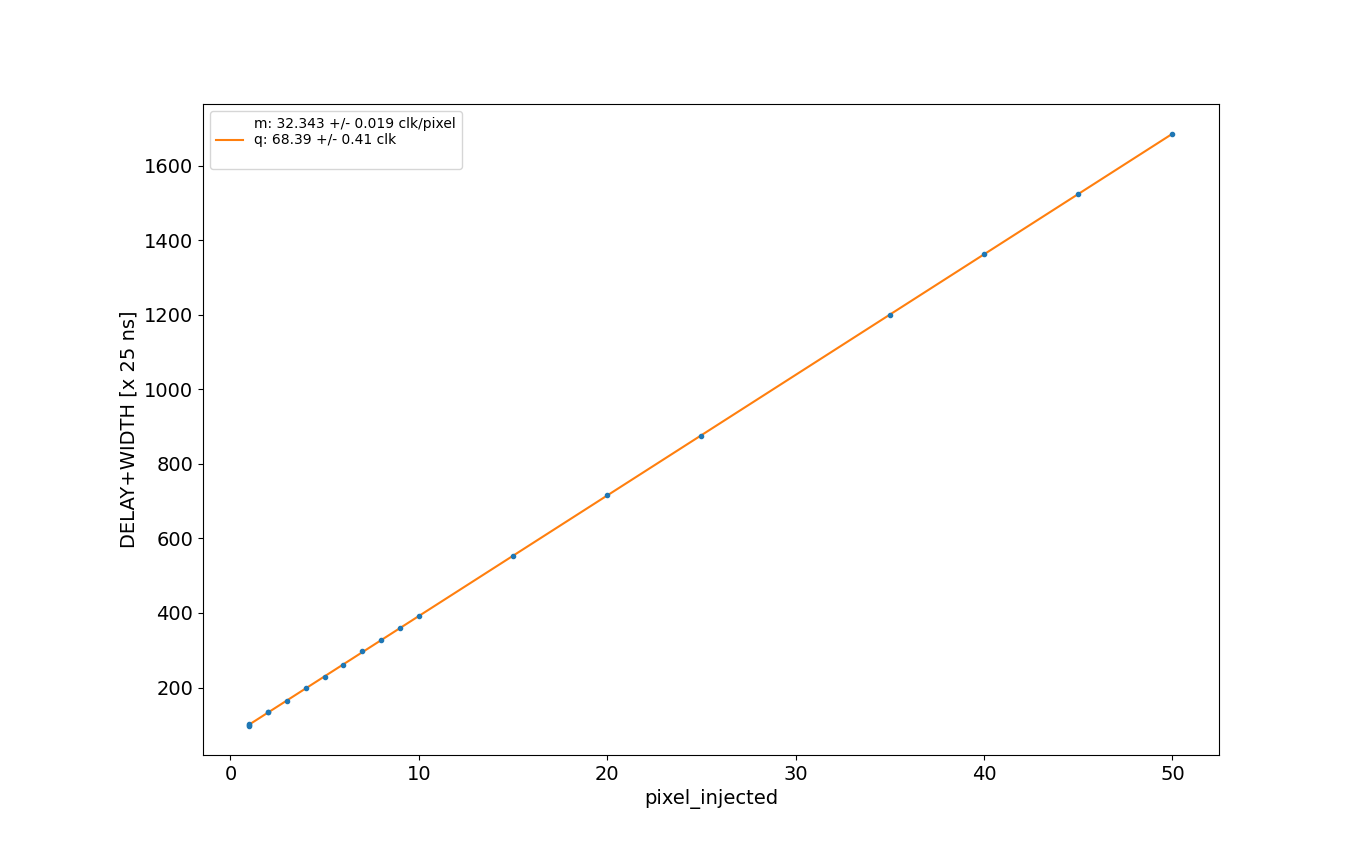
\includegraphics[width=.7\linewidth]{figures/Monopix1/dead_time.png}
                \caption{}
                \label{fig:dead_time}
            \end{figure}

    
